\documentclass[12pt, a4paper, twoside]{article}
\usepackage[utf8]{inputenc}
\usepackage{fancyhdr}
\usepackage{graphicx}
\usepackage{caption}
\usepackage{subcaption}
\usepackage[margin=1in,footskip=0.25in]{geometry}
\usepackage{pgf}
\usepackage[absolute, overlay]{textpos}
\usepackage{pdfpages}
\usepackage{circuitikz}
\setlength{\TPHorizModule}{1.0 pt}
\textblockorigin{\paperwidth}{0.0 pt}

\pagestyle{fancy}
\fancyhf{}
\lhead{Stromkreise \& Glühlampchen}
\rhead{Physik Bericht}
\begin{document}
    \pgfmathwidth{"\\\\ J. Dubois \& A. Huillet\\ MNG Rämibühl\\"}
    \begin{textblock}{\pgfmathresult}[1, 0](0, 0)
    \noindent
    \\\\ J. Dubois \& A. Huillet\\ MNG Rämibühl\\ 8001 Zürich
    \end{textblock}
    \begin{titlepage}

    \begin{center}
        \vspace*{8cm}
        \Huge
        \textbf{Stromkreise \& Glühlampchen}
 
        \vspace{0.5cm}
        \LARGE
        Physik Bericht  
    \end{center}
    \vspace*{8cm}
    \normalsize
    \hspace*{2cm}Physik Bericht mit Bezug auf das Praktikum vom 24. März 2022\\\\
    \hspace*{2cm}Zürich, 7. April 2022
    
             
 \end{titlepage}

    \newpage
    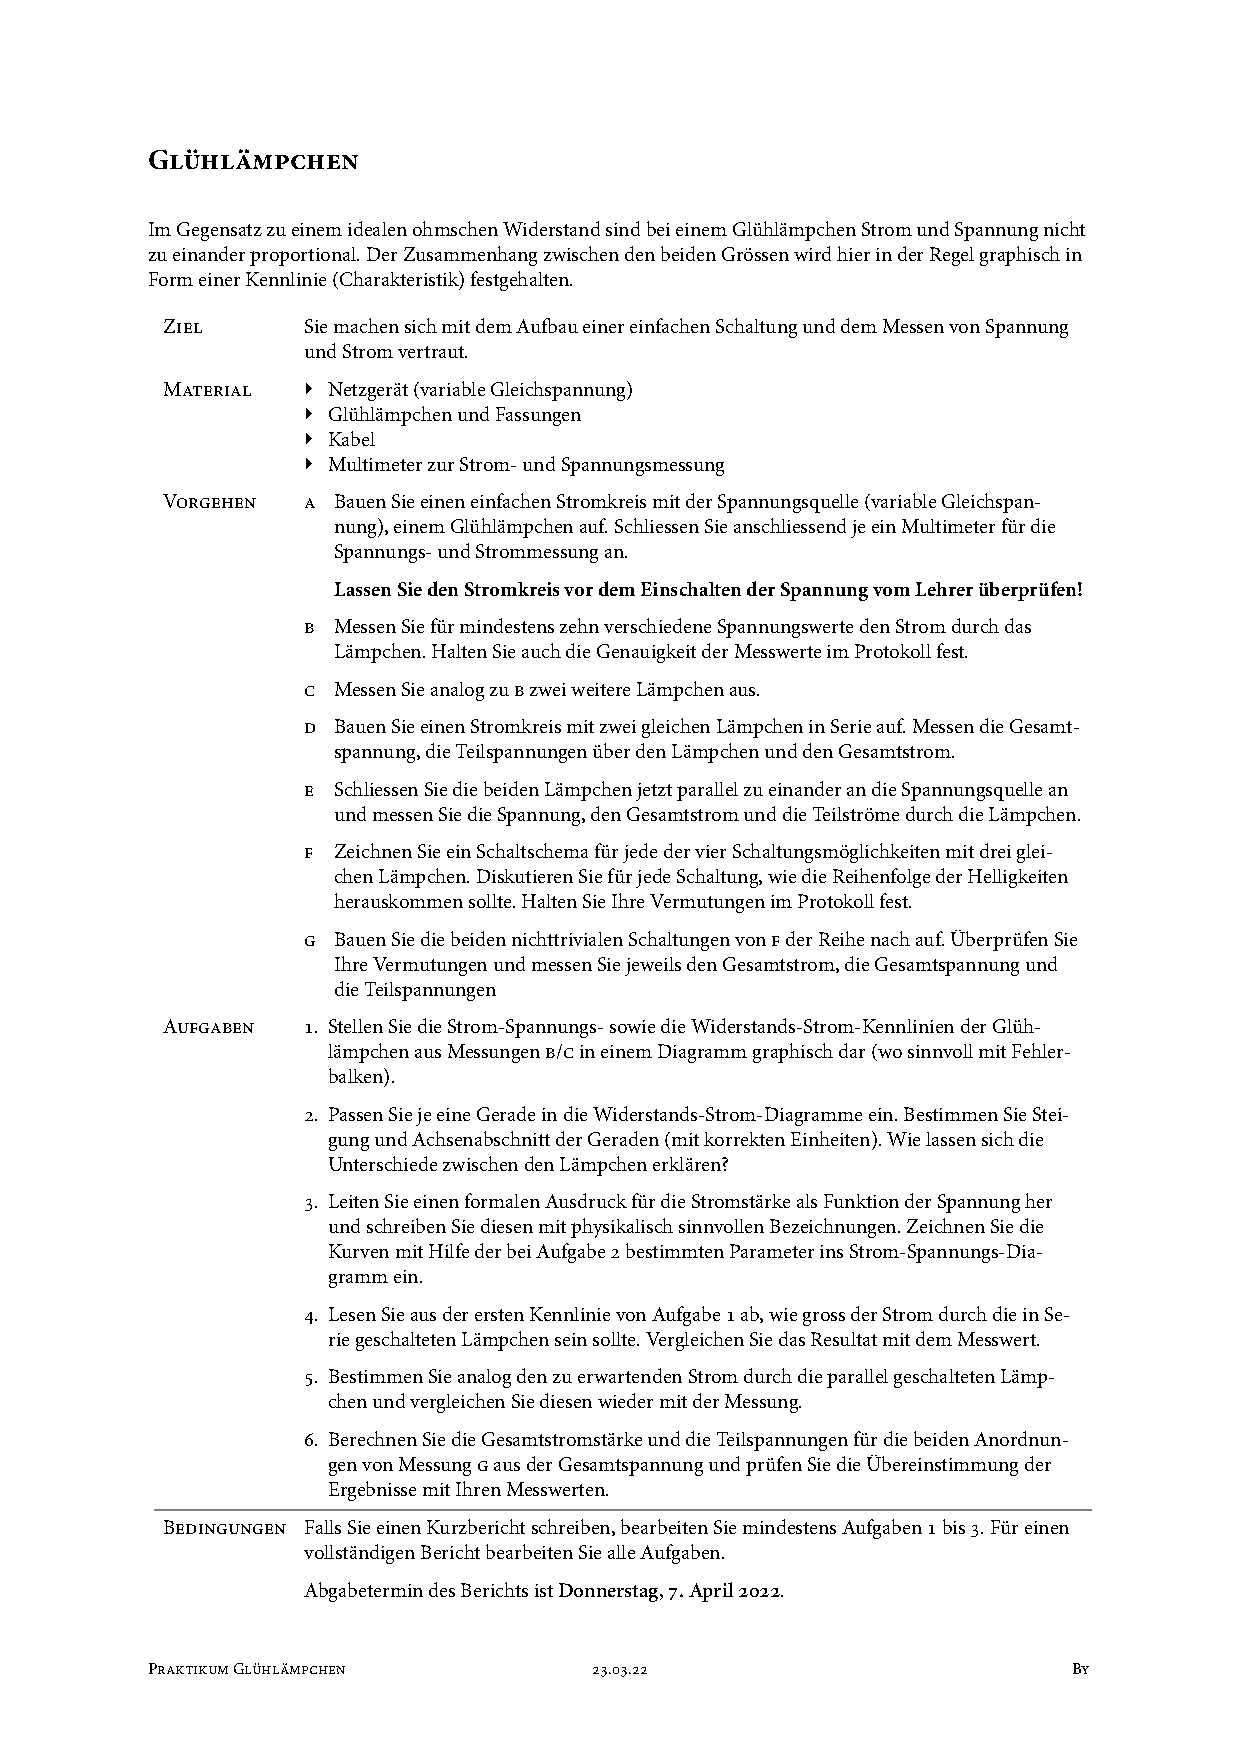
\includepdf[pages=-]{aufgabenstellung.pdf}
    \section{Einleitung}
    \newpage
    \section{Theorie}
    \newpage
    \section{Experiment}
    \newpage
    \section{Messungen}
    \subsection{Messung B}
    Bei Messung B wurden für zehn verschiedenen Spannungswerte den Strom durch das Lämpchen gemessen:\\
    \begin{center}
        \begin{tabular}{l|r}
            \textbf{Spannung U[V]} & \textbf{Stromstärke I[mA]}\\
            \hline
            3.65 & 39.50\\
            5.11 & 48.30\\
            8.33 & 64.60\\
            10.37 & 73.60\\
            12.50 & 82.20\\
            15.54 & 93.60\\
            17.62 & 100.70\\
            19.74 & 107.70\\
            23.80 & 120.00\\
            24.85 & 123.00
        \end{tabular}
    \end{center}
    \subsection{Messung C}
    In dieser Messung wurde das gleiche Verfahren wie bei Messung B bei zwei weiter Lämpchen angewendet.
    Messung für Lämpchen 2:\\
    \begin{center}
        \begin{tabular}{l|r}
            \textbf{Spannung U[V]} & \textbf{Stromstärke I[mA]}\\
            \hline
            
        \end{tabular}
    \end{center}
    Messung für Lämpchen 3:\\
    \begin{center}
        \begin{tabular}{l|r}
            \textbf{Spannung U[V]} & \textbf{Stromstärke I[mA]}\\
            \hline
        \end{tabular}
    \end{center}
    \subsection{Messung D}

    \subsection{Messung E}
    \subsection{Messung F}
    \subsection{Messung G}
    \newpage
    \section{Aufgaben}
    \newpage
    \section{Schlussfolgerungen}
    \newpage


\end{document}
